% DO NOT COMPILE THIS FILE DIRECTLY!
% This is included by the other .tex files.

\begin{frame}[t,plain]
\titlepage
\end{frame}

\begin{frame}
    \frametitle{about CIRCL and MISP}
    \begin{itemize}
        \item CIRCL
        \begin{itemize}
            \item National CERT for the for the private sector, communes, non-govermental entities in Luxembourg
            \item Government-driven initiative, funded by the ministry of economy
            \item Mission is to provide a systematic response facility to computer security threats and incidents
        \end{itemize}
        \item Our relationship with MISP has two sides
        \begin{itemize}
            \item We {\bf lead the development} of the MISP platform
            \item We are also involved with and {\bf run several communities}
        \end{itemize}
    \end{itemize}
\end{frame}

\begin{frame}
 \frametitle{MISP: Started from a practical use-case}
 \begin{itemize}
         \item During a malware analysis workgroup in 2012, we discovered that we worked on the analysis of the same malware.
         \item We wanted to share information in an easy and automated way {\bf to avoid duplication of work}.
         \item Christophe Vandeplas (then working at the CERT for the Belgian MoD) showed us his work on a platform that later became MISP.
         \item A first version of the MISP Platform was used by the MALWG and {\bf the increasing feedback of users} helped us to build an improved platform.
         \item MISP is now {\bf a community-driven development}.
 \end{itemize}
\end{frame}

\begin{frame}
\frametitle{What is MISP?}
\begin{itemize}
       \item MISP is a {\bf threat information sharing} platform that is free \& open source software
       \item A tool that {\bf collects} information from partners, your analysts, your tools, feeds
       \item Normalises, {\bf correlates}, {\bf enriches} the data
       \item Allows teams and communities to {\bf collaborate}
       \item {\bf Feeds} automated protective tools and analyst tools with the output
\end{itemize}
\end{frame}

\begin{frame}
\frametitle{Many objectives from different user-groups}
    \begin{itemize}
        \item Sharing indicators for a {\bf detection} matter.
            \begin{itemize}
                \item \textit{Do I have infected systems in my infrastructure or the ones I operate?}
            \end{itemize}
    \item Sharing indicators to {\bf block}.
            \begin{itemize}
                \item \textit{I use these attributes to block, sinkhole or divert traffic}
            \end{itemize}
    \item Sharing indicators to {\bf perform intelligence}.
            \begin{itemize}
                \item Gathering information about campaigns and attacks. \textit{Are they related? Who is targeting me? Who are the adversaries?}
            \end{itemize}
        \end{itemize}
        \vspace{1em}
        \begin{center}
        $\rightarrow$ These objectives can be {\bf conflicting}

        (e.g. False-positives have different impacts)
        \end{center}
    \end{frame}

\begin{frame}
\frametitle{Sharing Difficulties}
        \begin{itemize}
                \item Sharing difficulties are not really technical issues but often it's a matter of {\bf social interactions} (e.g. {\bf trust}).
                \item Legal restriction\footnote{\url{https://www.misp-project.org/compliance/}}
                        \begin{itemize}
                                \item \textit{Our legal framework doesn't allow us to share information}
                                \item \textit{Risk of information-leak is too high and it's too risky for our organization or partners.}
                        \end{itemize}
                \item Practical restriction
                        \begin{itemize}
                                \item \textit{We don't have information to share.}
                                \item \textit{We don't have time to process or contribute indicators.}
                                \item \textit{Our model of classification doesn't fit your model.}
                                \item \textit{Tools for sharing information are tied to a specific format, we use a different one.}
                        \end{itemize}
        \end{itemize}
\end{frame}


\begin{frame}
    \frametitle{MISP Project Overview}
    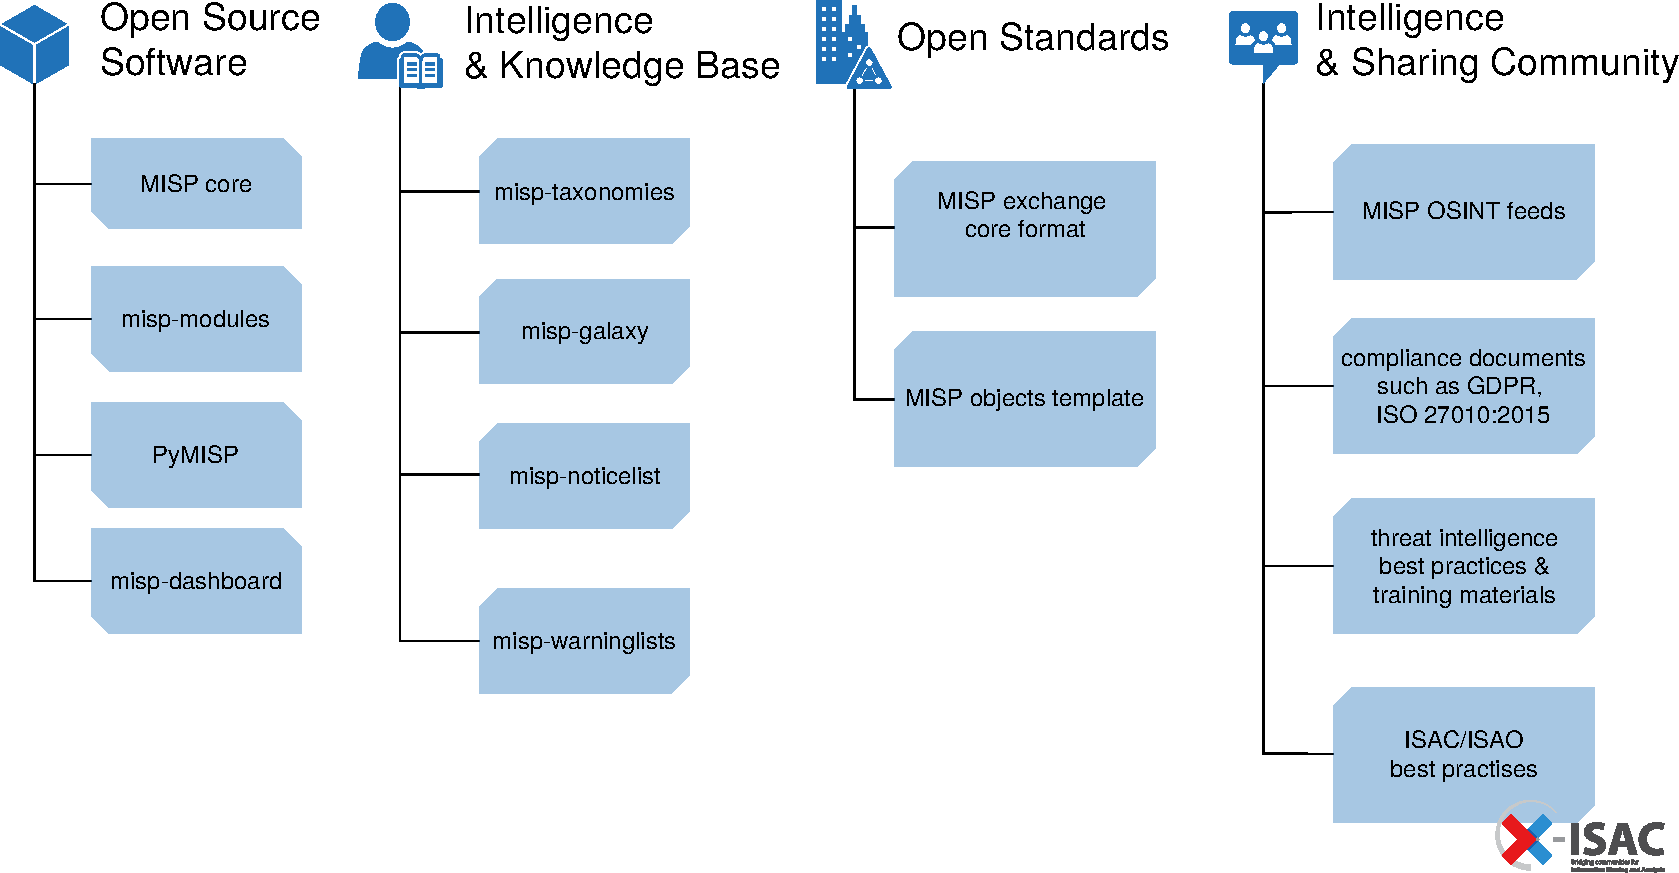
\includegraphics[scale=0.35]{misp-overview-simplified.pdf}
\end{frame}

\begin{frame}
    \frametitle{MISP model of governance}
    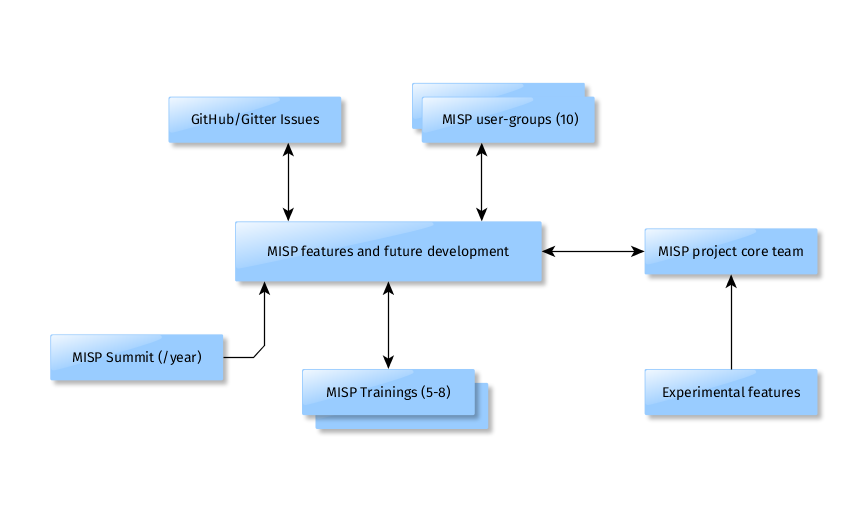
\includegraphics[scale=0.4]{governance.png}
\end{frame}

\begin{frame}
    \frametitle{Getting some naming conventions out of the way...}
     \begin{itemize}
            \item Data layer
            \begin{itemize}
                \item {\bf Events} are encapsulations for contextually linked information
                \item {\bf Attributes} are individual data points, which can be indicators or supporting data.
                \item {\bf Objects} are custom templated Attribute compositions
                \item {\bf Object references} are the relationships between other building blocks
            \end{itemize}
    \end{itemize}
\end{frame}

\begin{frame}
    \frametitle{Getting some naming conventions out of the way...}
     \begin{itemize}
            \item Context layer
            \begin{itemize}
                \item {\bf Tags} are labels attached to events/attributes and can come from {\bf Taxonomies}
                \begin{itemize}
                    \item \texttt{Android Malware}, \texttt{C2}, ...
                \end{itemize}

                \item {\bf Taxonomies} are a set of common classification allowing to express the same vocabulary among a distributed set of users and organisations 
                \begin{itemize}
                    \item \texttt{tlp:green}, \texttt{false-positive:risk="high"}, \texttt{gsma-fraud:technical="sim-card-cloning"}, \texttt{gsma-attack-category:spoofing}
                \end{itemize}

                \item {\bf Galaxy-clusters} are knowledge base items used to label events/attributes and come from {\bf Galaxies}. Basically a taxonomy with additional meta-information.
                \begin{itemize}
                    \item Typical {\bf Galaxy-clusters}: {\bf threat actors}, {\bf preventive measures}, ...
                    \item \texttt{misp-galaxy:bhadra-framework="Billing frauds"}, \texttt{misp-galaxy:bhadra-framework="DNS-based attacks"}, \texttt{misp-galaxy:threat-actor="APT 29"}
                \end{itemize}
            \end{itemize}
    \end{itemize}
\end{frame}

\begin{frame}
        \frametitle{A rich data-model: telling stories via relationships}
        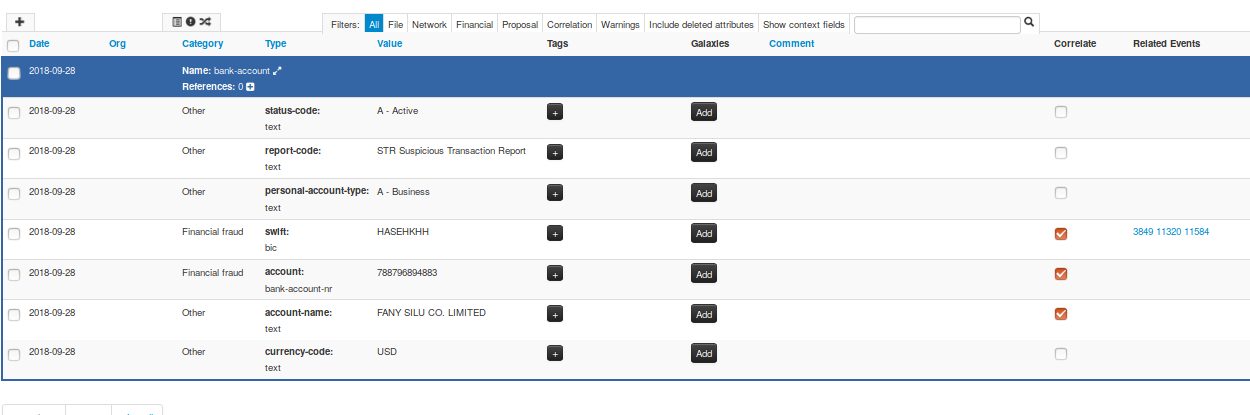
\includegraphics[scale=0.25]{screenshots/bankaccount.png}
        \begin{center}
            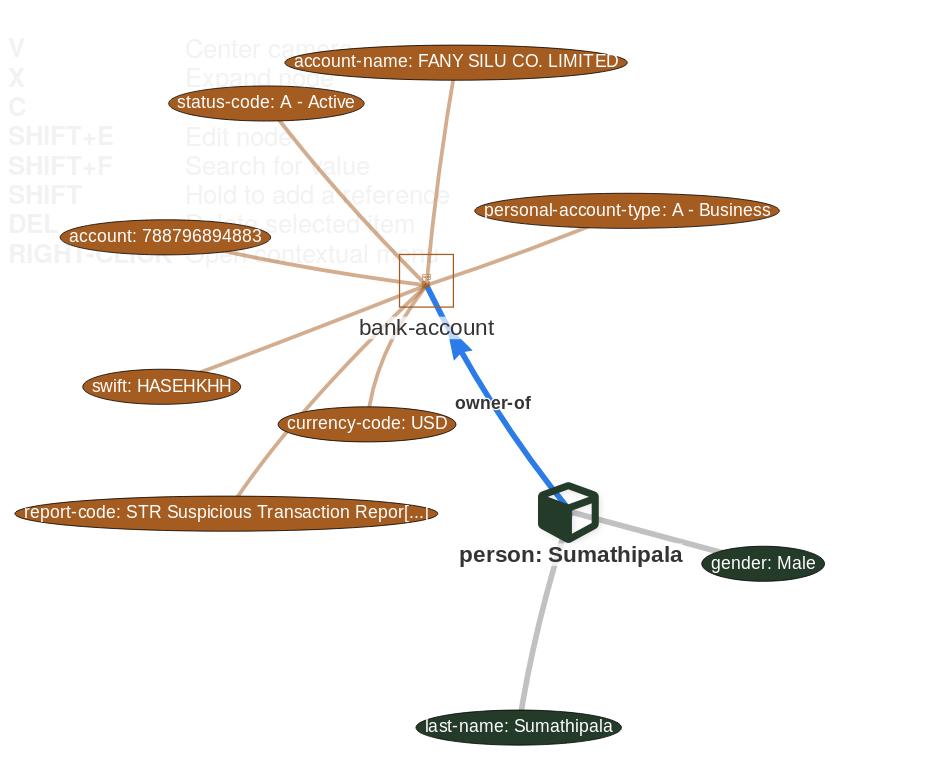
\includegraphics[scale=0.18]{screenshots/bankview.png}
        \end{center}
\end{frame}

\begin{frame}
        \frametitle{Correlation features: a tool for analysts}
        \begin{center}
            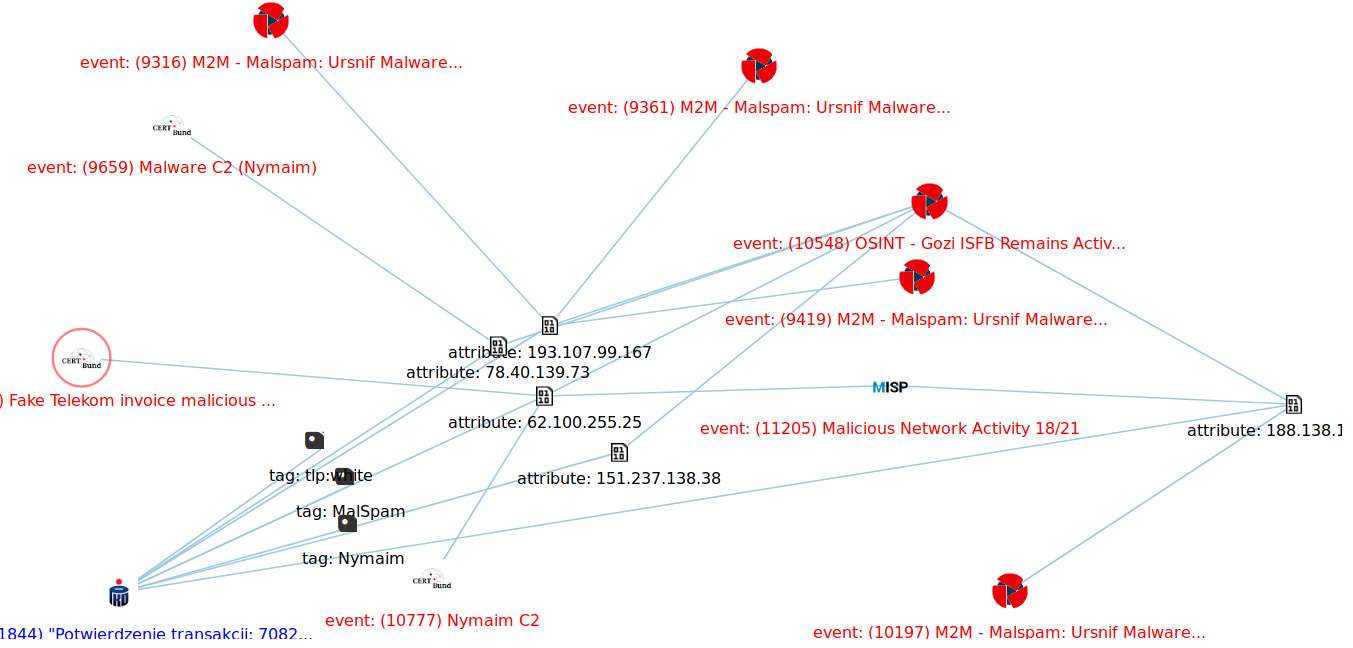
\includegraphics[scale=0.18]{screenshots/campaign.png}
        \end{center}
        \begin{itemize}
                \item To {\bf corroborate a finding} (e.g. is this the same campaign?), {\bf reinforce an analysis} (e.g. do other analysts have the same hypothesis?), {\bf confirm a specific aspect} (e.g. are the sinkhole IP addresses used for one campaign?) or just find if this {\bf threat is new or unknown in your community}.
        \end{itemize}
\end{frame}

\begin{frame}
        \frametitle{Contextualisation and aggregation}
        \begin{itemize}
                \item MISP integrates MITRE's Adversarial Tactics, Techniques, and Common Knowledge (ATT\&CK) and similar {\bf Galaxy Matrix}
        \end{itemize}
        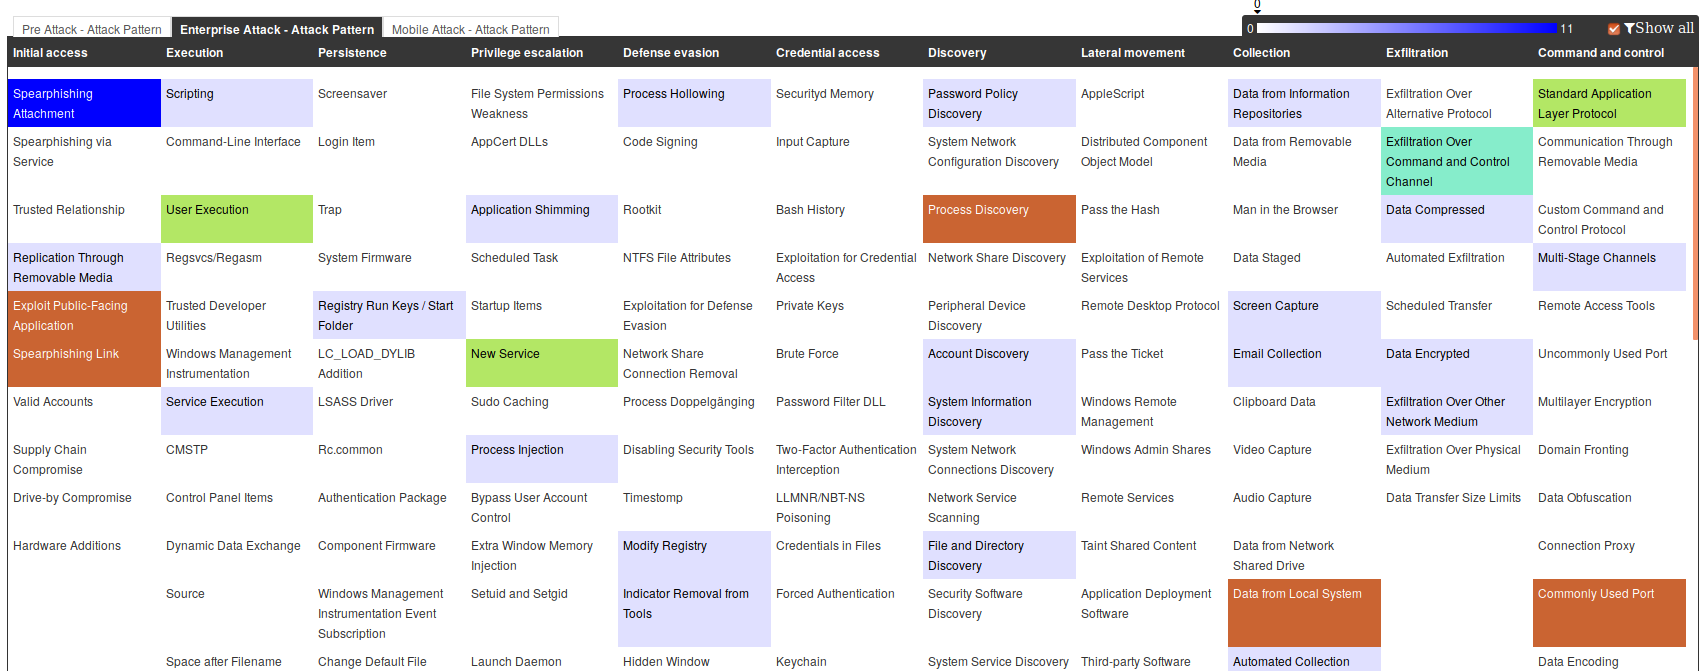
\includegraphics[scale=0.2]{screenshots/attack-screenshot.png}
\end{frame}

\begin{frame}
\frametitle{Sharing in MISP: Distribution}
    MISP offers granulars distribution settings:
    \begin{itemize}
        \item \texttt{Organisation only}
        \item \texttt{This community}
        \item \texttt{Connected communities}
        \item \texttt{All communities}
        \item Distribution lists - aka \texttt{\bf Sharing groups}
    \end{itemize}
    \begin{center}
    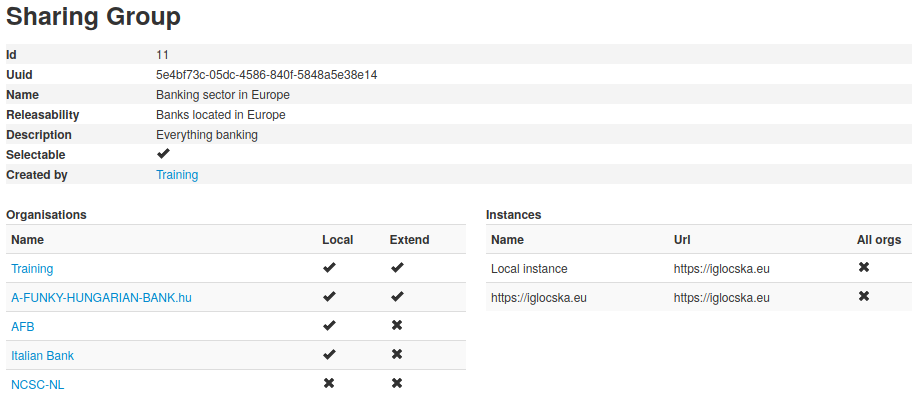
\includegraphics[scale=0.2]{screenshots/sg-example.png}
    \end{center}

    At multiple levels: Events, Attributes and Objects (and their Attributes)
\end{frame}

\begin{frame}
\frametitle{Sharing in MISP: Advanced usage}
    \begin{itemize}
        \item {\bf Delegation} for pseudo-anonymised information sharing
        \item {\bf Proposals} and {\bf Extended events} for collaborated information sharing
        \item 2-way synchronisation, Feed system, air-gapped sharing
        \item User defined {\bf filtered sharing} for all the above mentioned methods
        \item Cross-instance information {\bf caching} for quick lookups of large data-sets
        \item Support for multi-MISP internal enclaves
    \end{itemize}
\end{frame}

\begin{frame}
\frametitle{MISP core distributed sharing functionality}
    \begin{itemize}
        \item MISP's core functionality is sharing where everyone can be a consumer and/or a contributor/producer.
        \item Quick benefit without the obligation to contribute.
        \item Low barrier access to get acquainted to the system.
    \end{itemize}
    \begin{center}
        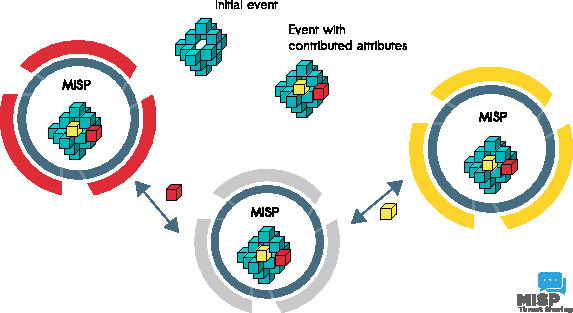
\includegraphics[scale=0.9]{misp-distributed.pdf}
    \end{center}
\end{frame}



\begin{frame}
\frametitle{Information quality management}
    \begin{itemize}
        \item Correlating data
        \item Feedback loop from detections via {\bf Sightings}
        \item {\bf False positive management} via the warninglist system
        \item {\bf Enrichment system} via MISP-modules
        \item {\bf Integrations} with a plethora of tools and formats
        \item Flexible {\bf API} and support {\bf libraries} such as PyMISP to ease integration
        \item {\bf Timelines} and giving information a temporal context
        \item Full chain for {\bf indicator life-cycle management}
    \end{itemize}
\end{frame}


\begin{frame}
        \frametitle{Sightings support}
        \begin{columns}[t]
        \column{5.0cm}
        \begin{figure}
        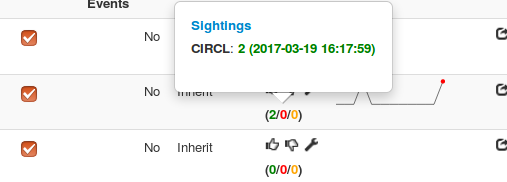
\includegraphics[scale=0.3]{screenshots/sighting-n.png}\\
        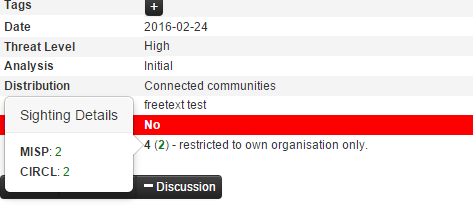
\includegraphics[scale=0.34]{screenshots/Sightings2.PNG}
        \end{figure}
        \column{7cm}
        \begin{itemize}
                \item \textit{Has a data-point been {\bf sighted} by me or the community before?}
                \item Additionally, the sighting system supports negative sigthings (FP) and expiration sightings.
                \item Sightings can be performed via the API or the UI.
                \item Many use-cases for {\bf scoring indicators} based on users sighting.
                \item For large quantities of data, {\bf SightingDB} by Devo
        \end{itemize}
        \end{columns}
\end{frame}

\begin{frame}
  \frametitle{Timelines and giving information a temporal context}
  \begin{itemize}
    \item Recently introduced {\bf \texttt{first\_seen}} and {\bf \texttt{last\_seen}} data points
    \item All data-points can be placed in time
    \item Enables the {\bf visualisation} and {\bf adjustment} of indicators timeframes 
  \end{itemize}
  \begin{center}
    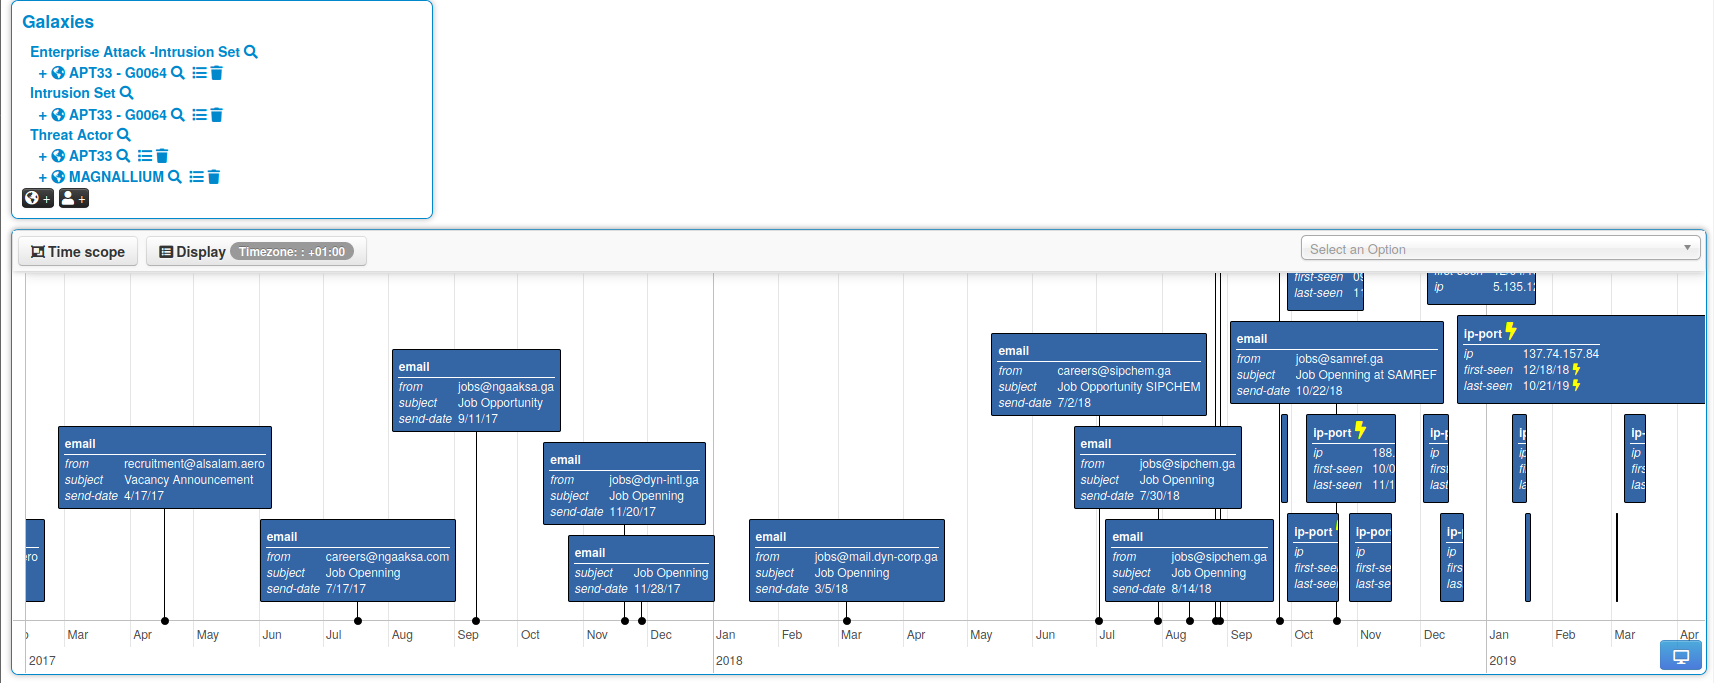
\includegraphics[width=1.0\linewidth]{timeline-misp-overview.png}
  \end{center}
\end{frame}

\begin{frame}
    \frametitle{Life-cycle management via decaying of indicators}
    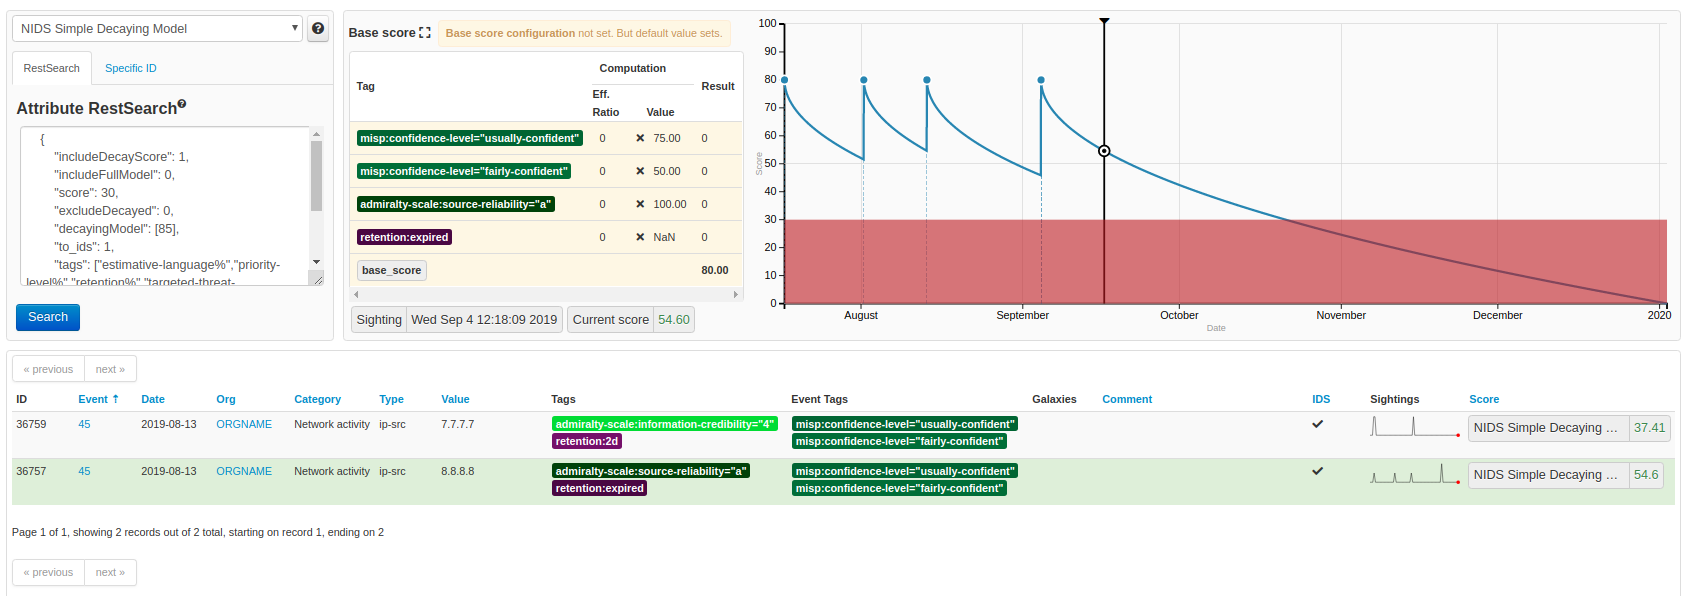
\includegraphics[width=1.00\linewidth]{decaying-simulation.png}
    Expiration based on user-defined \textit{Models}
\end{frame}

\begin{frame}
\frametitle{DFIR and MISP digital evidences}
        \begin{itemize}
                \item {\bf Share analysis and report} of digital forensic evidences.
                \item {\bf Propose changes} to existing analysis or report.
                \item Extending existing event with additional evidences for local or limited use (sharing can be defined at event level or attribute level).
                \item {\bf Evaluate correlations}\footnote{MISP has a flexible correlation engine which can correlate on 1-to-1 value but also fuzzy hashing (e.g. ssdeep) or CIDR block matching.} of evidences against external or existing attributes.
                \item {\bf Report sighting} such as false-positive or true-positive (e.g. a partner/analyst has seen a similar indicator).
        \end{itemize}
\end{frame}

\begin{frame}
\frametitle{Benefits of using MISP}
\begin{itemize}
        \item  LE can leverage the long-standing experience in information sharing and {\bf bridge their use-cases} with MISP's information sharing mechanisms.
        \item {\bf Accessing existing MISP information sharing communities} by getting actionable information from CSIRTs/CERTs networks or security researchers.
        \item {\bf Bridging LE communities with other communities}. Sharing groups can be created (and managed) between cross-sectors to support specific use-cases.
        \item {\bf MISP standard format} is a flexible format which can be extended by the users who use the MISP platform. A MISP object template can be created in 30 minutes and directly share information with your model towards existing communities.
\end{itemize}
\end{frame}

\begin{frame}
        \frametitle{Future of Information Sharing}
        \begin{itemize}
        \item MISP is a long-term project (started in 2012) and since {\bf information sharing is becoming more essential} than ever to thwart threats, we have long-term plans for the project as the project is used in various critical information exchange communities
        \item We hope to have the means to be the enablers and the interface for real cross-sectorial sharing and support the organisations facing hybrid threats
        \item Tools, open standards and interoperable software (e.g. DFIR tools) are driving forces behind resilient information exchange communities
        \item Getting ideas and practical {\bf use-cases from LE community} is vital, don't hesitate to contact us
        \end{itemize}
\end{frame}


\begin{frame}
  \frametitle{Get in touch if you have any questions}
  \begin{itemize}
    \item Contact CIRCL
    \begin{itemize}
      \item info@circl.lu
      \item \url{https://twitter.com/circl_lu}
      \item \url{https://www.circl.lu/}
    \end{itemize}
    \item Contact MISPProject
    \begin{itemize}
      \item \url{https://github.com/MISP}
      \item \url{https://www.misp-project.org/}
      \item \url{https://twitter.com/MISPProject}
    \end{itemize}
  \end{itemize}
\end{frame}

